\documentclass[11pt, a4paper]{article}

\usepackage[a4paper, top=2.5cm, bottom=2.5cm, left=2.5cm, right=2.5cm]{geometry}
\usepackage{amsmath}
\usepackage{graphicx}
\usepackage{booktabs}
\usepackage{parskip}
\usepackage{fancyhdr}
\usepackage{titlesec}
\usepackage{xcolor}
\usepackage{mdframed}
\usepackage{hyperref}
\usepackage{caption}
\usepackage{float}

\hypersetup{colorlinks=true, linkcolor=black, urlcolor=blue}

\pagestyle{fancy}
\fancyhf{}
\renewcommand{\headrulewidth}{0.4pt}
\renewcommand{\footrulewidth}{0.4pt}
\fancyhead[L]{\small\textit{Study Notes: C-MAPSS Operating Conditions}}
\fancyhead[R]{\small\thepage}
\fancyfoot[C]{\small\textit{``I'm not stupid, I'm just slow''}}

\titleformat{\section}{\large\bfseries}{}{0em}{}[\titlerule]
\titleformat{\subsection}{\normalsize\bfseries}{}{0em}{}

\newmdenv[
  backgroundcolor=gray!8,
  linecolor=gray!40,
  linewidth=0.8pt,
  innerleftmargin=10pt, innerrightmargin=10pt,
  innertopmargin=8pt,   innerbottommargin=8pt,
  skipabove=8pt, skipbelow=8pt
]{keybox}

\newmdenv[
  backgroundcolor=orange!6,
  linecolor=orange!40,
  linewidth=0.8pt,
  innerleftmargin=10pt, innerrightmargin=10pt,
  innertopmargin=8pt,   innerbottommargin=8pt,
  skipabove=8pt, skipbelow=8pt
]{insightbox}

\captionsetup{font=small, labelfont=bf, skip=4pt}

% -------------------------------------------------------------------
\begin{document}
% -------------------------------------------------------------------

{\Large\bfseries C-MAPSS Operating Conditions}

\smallskip
{\small Saxena et al., PHM'08 \quad --- \quad
Sub-datasets FD002 and FD004 \quad --- \quad
\textit{Working reference}}

\medskip\hrule\medskip

\tableofcontents

\bigskip\hrule\bigskip

% -------------------------------------------------------------------
\section{What Are Operating Conditions?}
% -------------------------------------------------------------------

A turbofan engine does not always operate at the same altitude,
speed, and throttle setting. During a single flight it passes
through multiple distinct phases --- takeoff, climb, cruise,
and descent. Each phase demands different engine behaviour and
produces different sensor readings.

In C-MAPSS, an \textbf{operating condition} is one specific
combination of three variables:

\begin{center}
\small
\begin{tabular}{@{}llp{8cm}@{}}
  \toprule
  Column & Physical quantity & Description \\
  \midrule
  \texttt{op\_setting\_1} & Altitude &
    Height above sea level. Stored as \emph{thousands of feet}
    in the file. Range: 0 to 42{,}000\,ft. \\[4pt]
  \texttt{op\_setting\_2} & Mach number &
    Flight speed as a fraction of the speed of sound.
    Dimensionless. Range: 0 to 0.84. \\[4pt]
  \texttt{op\_setting\_3} & TRA &
    Throttle Resolver Angle, in degrees.
    The physical angle of the pilot's throttle lever.
    Range: 20° to 100°. \\
  \bottomrule
\end{tabular}
\end{center}

The paper states the ranges but does not list the six exact
combinations. They are recovered from the data by
KMeans clustering on the three \texttt{op\_setting} columns
(see Section~\ref{sec:kmeans}).

% -------------------------------------------------------------------
\section{The Throttle Resolver Angle (TRA)}
% -------------------------------------------------------------------

TRA is the most intuitive of the three variables. It is the
physical angle of the throttle lever on the flight deck ---
like a car accelerator pedal, but measured as an angle rather
than displacement. A resolver (rotary sensor) reads the lever
position and sends it to the engine controller.

\begin{center}
\small
\begin{tabular}{@{}ccp{8cm}@{}}
  \toprule
  TRA & Thrust level & Meaning \\
  \midrule
  0°   & Idle    & Engine at minimum power. \\
  60°  & Reduced & Partial thrust. Used for fuel-efficient cruise. \\
  100° & Maximum & Full commanded thrust. \\
  \bottomrule
\end{tabular}
\end{center}

\begin{insightbox}
\textbf{Why is TRA = 100° at high altitude?}
At 42{,}000\,ft the air density is roughly 20\% of sea level.
The engine must work at full throttle just to maintain cruise
thrust --- there are simply not enough air molecules to produce
adequate thrust at reduced settings. So counterintuitively,
the highest altitudes require the highest TRA.

The one exception is C3 (25{,}000\,ft, TRA = 60°) --- a
mid-altitude cruise phase where the aircraft can afford to
reduce fuel burn without falling below minimum cruise thrust.
\end{insightbox}

% -------------------------------------------------------------------
\section{The Six Conditions}
% -------------------------------------------------------------------

FD002 and FD004 simulate an engine cycling through six distinct
flight conditions within each engine life. Every engine visits
all six conditions --- the order is random from cycle to cycle.

The following four charts examine the conditions from every
angle, one variable pair at a time.

% -------------------------------------------------------------------
\subsection{Chart A --- Altitude vs Mach number}
% -------------------------------------------------------------------

\begin{figure}[H]
  \centering
  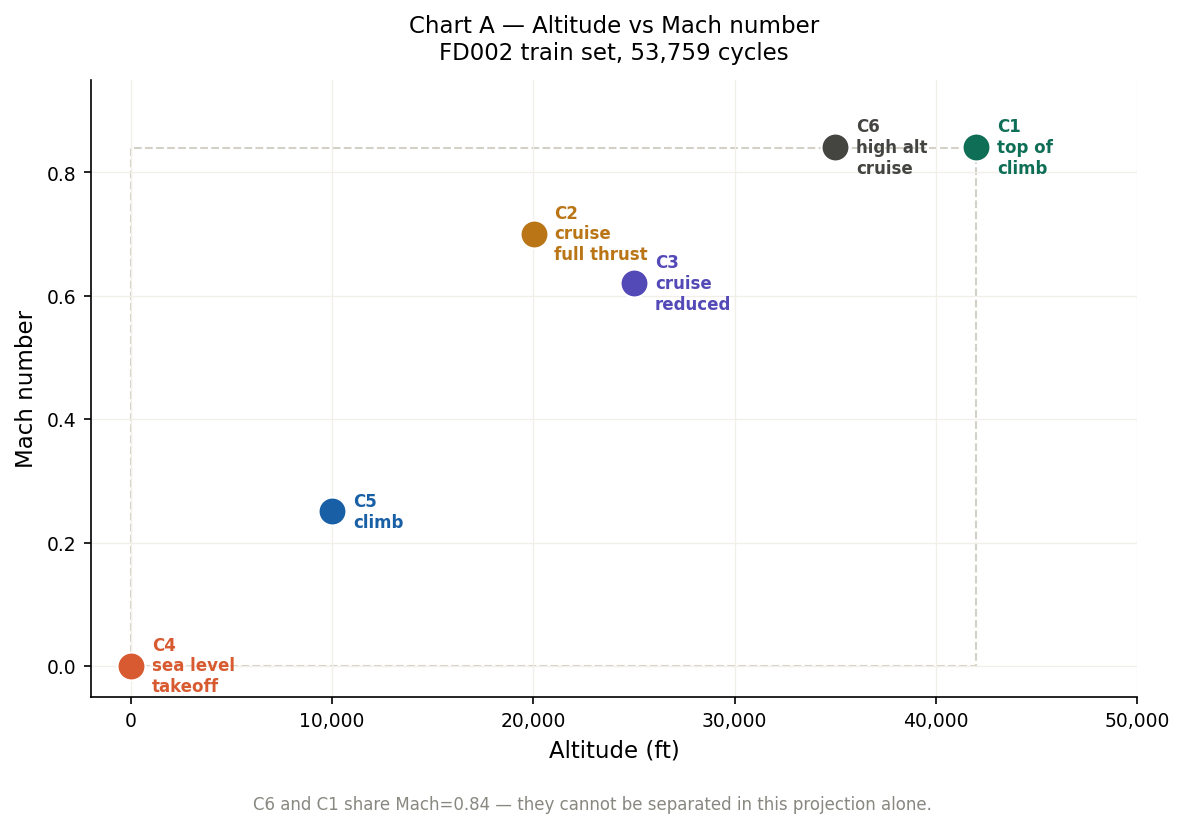
\includegraphics[width=0.92\textwidth]{cond_A_alt_mach.png}
  \caption{Altitude vs Mach number. The dashed box is the
  paper-stated range (alt 0--42{,}000\,ft, Mach 0--0.84).
  Five of six conditions are clearly separated.
  C6 and C1 share Mach = 0.84 and appear close together ---
  altitude alone separates them (35{,}000 vs 42{,}000\,ft).}
  \label{fig:chartA}
\end{figure}

Reading Chart~A left to right traces the flight profile:
C4 at the origin (sea level, stationary), C5 at low altitude
climbing, C2/C3 at mid-cruise, and C6/C1 at high altitude.
The general trend is diagonal --- higher altitude correlates
with higher speed, as expected in aviation.

% -------------------------------------------------------------------
\subsection{Chart B --- Altitude vs TRA}
% -------------------------------------------------------------------

\begin{figure}[H]
  \centering
  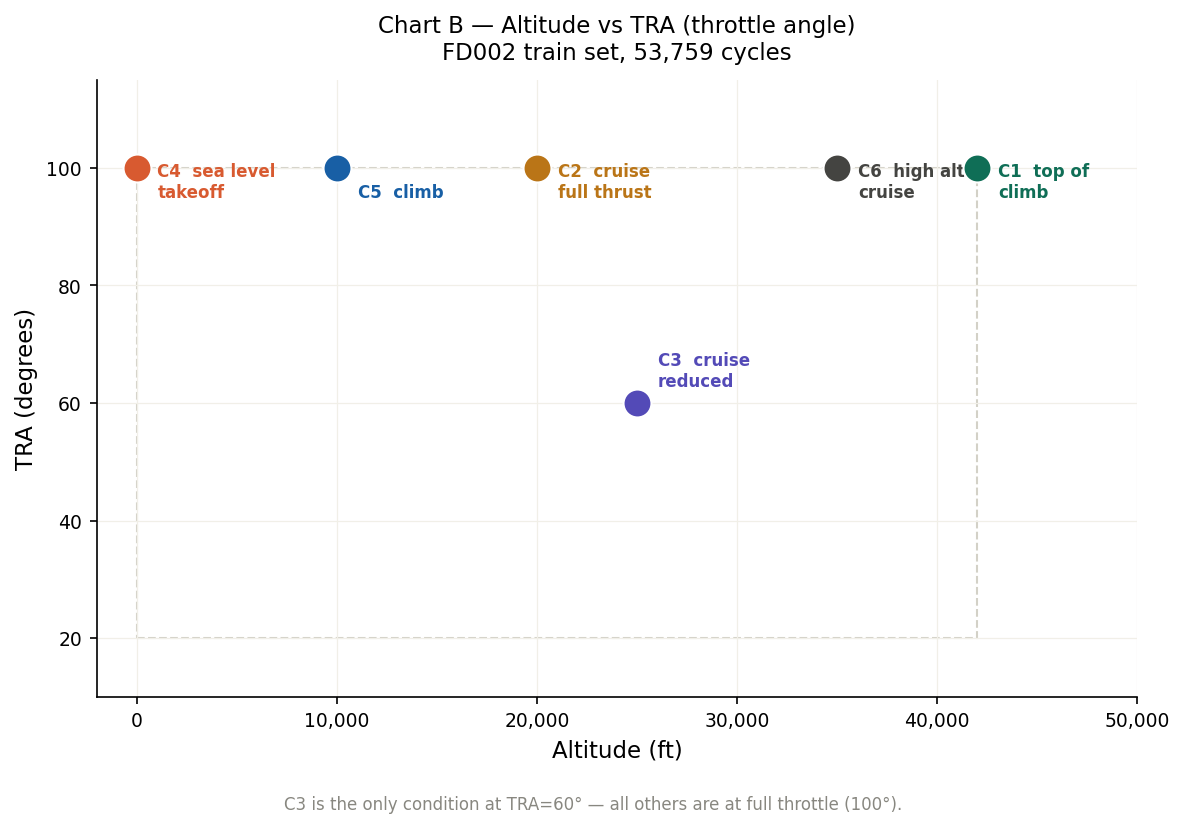
\includegraphics[width=0.92\textwidth]{cond_B_alt_tra.png}
  \caption{Altitude vs TRA (throttle resolver angle).
  Five conditions sit on a flat line at TRA = 100° (full throttle).
  C3 is the only outlier at TRA = 60°, at 25{,}000\,ft.
  This is the most visually striking separation in the dataset.}
  \label{fig:chartB}
\end{figure}

Chart~B directly answers the question ``why is TRA almost
always 100°?'' The flat horizontal line at TRA = 100° shows
that across sea level takeoff, climb, and all high-altitude
phases, the engine is at full commanded thrust. Only C3 ---
the mid-altitude reduced-thrust cruise --- breaks the pattern.

% -------------------------------------------------------------------
\subsection{Chart C --- Mach number vs TRA}
% -------------------------------------------------------------------

\begin{figure}[H]
  \centering
  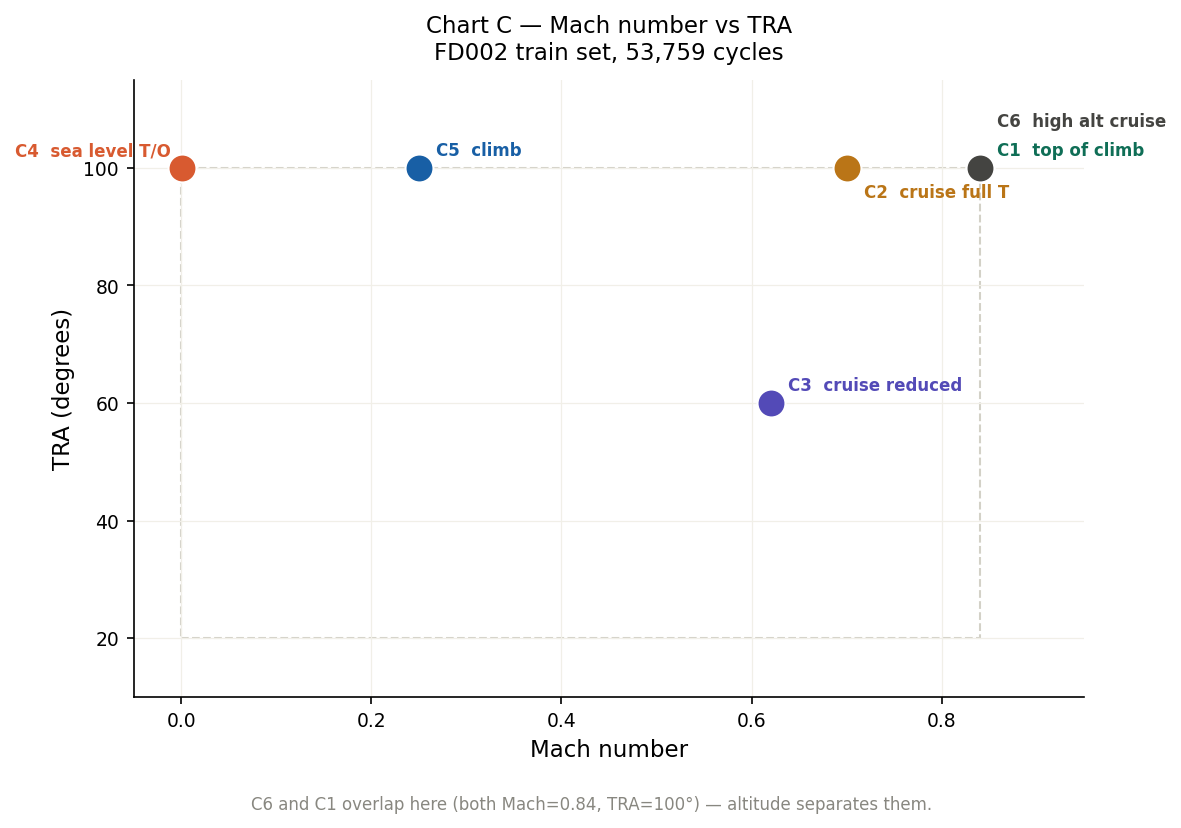
\includegraphics[width=0.92\textwidth]{cond_C_mach_tra.png}
  \caption{Mach number vs TRA. C6 and C1 overlap exactly
  (both at Mach = 0.84, TRA = 100°). In this projection they
  are indistinguishable. Only altitude (Chart~A) separates them.
  This demonstrates why all three \texttt{op\_setting} columns
  are needed for clustering.}
  \label{fig:chartC}
\end{figure}

Chart~C reveals the fundamental reason why KMeans is run on
all three columns simultaneously. No single 2D projection
cleanly separates all six conditions. C6 and C1 are identical
in Mach and TRA --- altitude is the only distinguishing
dimension. A 2D clustering on any two columns alone would
merge them into one cluster.

% -------------------------------------------------------------------
\subsection{Chart D --- Centroid reference table}
% -------------------------------------------------------------------

\begin{figure}[H]
  \centering
  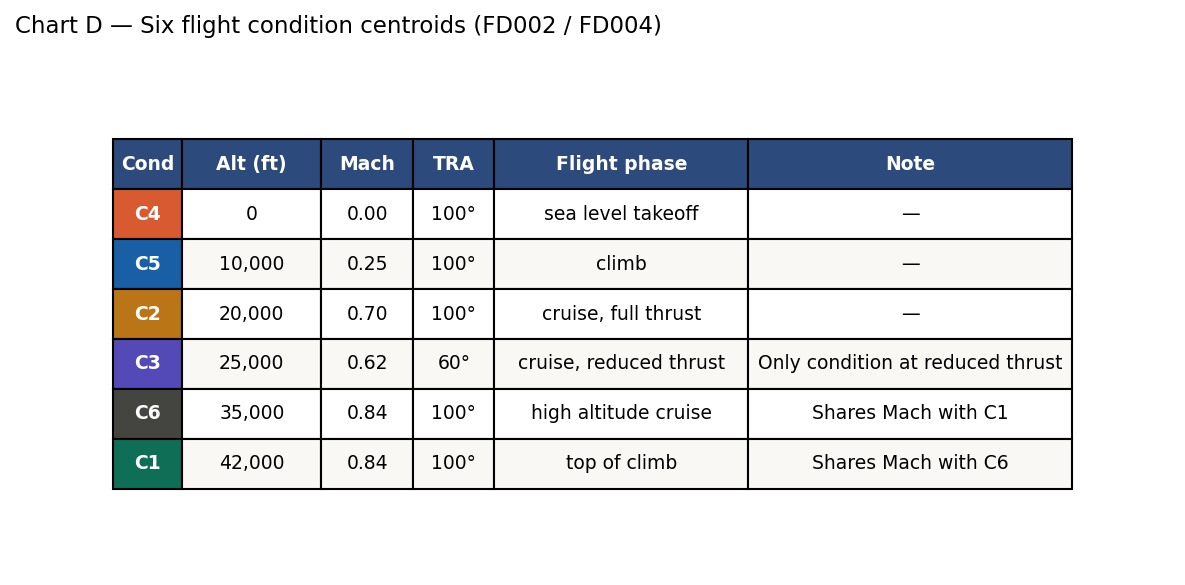
\includegraphics[width=\textwidth]{cond_D_table.png}
  \caption{Complete centroid reference for all six conditions.
  The Note column highlights which conditions share a dimension
  with another, explaining why 3D clustering is required.}
  \label{fig:chartD}
\end{figure}

% -------------------------------------------------------------------
\section{Why Only FD002 and FD004?}
% -------------------------------------------------------------------

FD001 and FD003 simulate a single operating condition --- sea
level only. All rows have \texttt{op\_setting\_1} = 0,
\texttt{op\_setting\_2} = 0, \texttt{op\_setting\_3} = 100.

This makes them simpler --- sensor readings are directly
comparable across cycles without any condition-wise
normalisation. The \texttt{condition\_id} = 1 for every row
and carries no information.

% -------------------------------------------------------------------
\section{How the Six Conditions Are Recovered}
\label{sec:kmeans}
% -------------------------------------------------------------------

The six exact combinations are recovered by KMeans clustering
($k = 6$) on the three \texttt{op\_setting} columns.
The algorithm minimises:

\begin{equation}
  J = \sum_{i=1}^{n} \left\| x_i - \mu_{c(i)} \right\|^2
\end{equation}

where $x_i = (\texttt{op\_setting\_1}_i,\,
\texttt{op\_setting\_2}_i,\, \texttt{op\_setting\_3}_i)$
and $\mu_k$ is the centroid of cluster $k$.

Because the simulator snaps to exactly six discrete flight
points (with only tiny noise), inertia is near zero
($J \approx 0.41$ for FD002). The centroid of each cluster
is the exact flight point, not an approximation.

\begin{keybox}
\textbf{Label ordering warning.} Condition labels (C1--C6)
are assigned by KMeans in arbitrary order. The same physical
condition may receive a different label in FD002 vs FD004.
Always compare conditions by \texttt{op\_setting} values,
never by label number.
\end{keybox}


% -------------------------------------------------------------------
\section{What Is a Centroid, and Why Does It Matter Here?}
% -------------------------------------------------------------------

\subsection{The general idea}

A \textbf{centroid} is the centre of a cluster --- the point
that minimises the average distance to all members of that cluster.
Geometrically it is the mean position of all points assigned
to the cluster.

In a typical clustering problem, data points are spread in
fuzzy clouds. The centroid sits somewhere inside the cloud ---
it is an approximation, not an actual data point. Figure~\ref{fig:discrete}
shows the contrast between the typical case and what happens
in C-MAPSS.

\begin{figure}[H]
  \centering
  
\includegraphics[width=\textwidth]{20_kmeans_discrete_points.png}
  \caption{Left: typical clustering --- data spreads in fuzzy clouds,
  centroids are approximations (shown with dashed circles).
  Right: C-MAPSS --- all data snaps to exactly 6 discrete flight
  points. The centroid coincides exactly with the data point.
  Inertia = 0.41 (near zero) confirms this.}
  \label{fig:discrete}
\end{figure}

\subsection{Why C-MAPSS centroids are exact}

The C-MAPSS simulator always sets the engine to one of exactly
six predetermined flight conditions before recording each cycle.
Every row in the dataset therefore has \texttt{op\_setting}
values that are essentially identical to one of the six target
points --- with only tiny sensor noise ($\pm$0.001 or less).

When KMeans clusters these points, each cluster contains
thousands of rows that all sit at almost exactly the same
3D coordinate. The mean of those rows --- the centroid ---
lands at that coordinate. There is no approximation because
there is no spread to approximate.

\subsection{The four algorithm steps}

Figure~\ref{fig:steps} shows what KMeans actually does on
this data, step by step.

\begin{figure}[H]
  \centering
  
\includegraphics[width=\textwidth]{21_kmeans_algorithm_steps.png}
  \caption{KMeans in four steps on C-MAPSS data.
  Step 1: place 6 centroids randomly (X marks).
  Step 2: assign each data point to its nearest centroid
  (color = assigned cluster, dashed lines show assignment).
  Step 3: recompute each centroid as the mean of its cluster
  (arrows show centroids moving toward the true flight points).
  Step 4: converged --- centroid sits exactly on the data point,
  inertia $\approx$ 0.}
  \label{fig:steps}
\end{figure}

The key observation from Step 4: the centroid ring and the
data dot coincide. This is not a coincidence --- it is a
consequence of the discrete simulator design. In a real-world
vibration or wear dataset, you would never see this. The
C-MAPSS data is unusually clean precisely because it is
a digital twin, not real sensor data.

\subsection{Why the label numbers seem random}

Looking at Chart D, the conditions sorted by altitude are
C4, C5, C2, C3, C6, C1 --- not C1, C2, C3, C4, C5, C6.
This is because KMeans assigns label numbers by the order
in which centroids happened to converge in that particular
run, not by altitude or any physical property.

\begin{keybox}
\textbf{The label number has no physical meaning.}
C1 does not mean ``lowest altitude'' or ``first condition''.
It simply means ``whichever cluster was internally labelled 0
by the KMeans run on that sub-dataset''. Two sub-datasets
run independently (FD002 and FD004) will produce different
label assignments for the same physical conditions.
Always trace a condition back to its \texttt{op\_setting}
values to know what it physically represents.
\end{keybox}


% -------------------------------------------------------------------
\section{Why Operating Conditions Matter for Analysis}
% -------------------------------------------------------------------

Raw sensor values are not comparable across conditions.
Fan inlet temperature $T_2$ at sea level is hundreds of
degrees Rankine higher than at 42{,}000\,ft --- purely due
to altitude, not engine health. Feeding raw values into a
model trains it to recognise flight conditions rather than
degradation.

The solution is condition-wise normalisation:

\begin{equation}
  x_{\text{norm}} = \frac{x - \mu_{s,c}}{\sigma_{s,c}}
\end{equation}

where $\mu_{s,c}$ and $\sigma_{s,c}$ are computed from
healthy (early-life) cycles at condition $c$ only.
After this step each value expresses deviation from the
healthy baseline at that specific flight condition.

\begin{keybox}
\textbf{Summary.}
\begin{itemize}
  \item FD001/FD003: one condition, global normalisation sufficient.
  \item FD002/FD004: six conditions, condition-wise normalisation required.
  \item \texttt{condition\_id} identifies the condition per cycle.
  \item No 2D projection separates all six conditions ---
        all three \texttt{op\_setting} columns are needed.
  \item Labels are not comparable across sub-datasets.
\end{itemize}
\end{keybox}

% -------------------------------------------------------------------
\end{document}
